%%%%%%%%%%%%%%%%%%%%%%%%%%%%%%%%%%%%%%%%%%%%
%
% 2.1.2: Delta-Sigma Performance Criteria
%
%%%%%%%%%%%%%%%%%%%%%%%%%%%%%%%%%%%%%%%%%%%%


%%%%%%%%%%%%%%%%%%%%%%%%%%%%%%%%%%%%%%%%%%%%
%%% 2.1.2.1 Random Processes

\subsubsection{Signal and Noise Power}
Several data converter performance metrics are a function of the output signal power and
output noise power contained in the collective output signal. Because output signals are
modelled deterministically the signal power is defined as follows.
%----------------------
\begin{equation}\label{eq:signal_power}
 P_s
 =\begin{cases}
\displaystyle\sum_{i=-\infty}^{\infty}{\bigl|x(i)\bigr|^2}, \qquad\text{Discrete
process}\\
\displaystyle\int_{-\infty}^{\infty}{\bigl|x(t)\bigr|^2}dt, \quad\text{Continuous
process}
       \end{cases}
\end{equation}
%----------------------
However, because noise is modelled as a random process, noise power can be defined  as
$$P_n=E[x^2]$$
where $E[\cdot]$ is the expectation or mean and is defined as follows.
%----------------------
\begin{equation}\label{eq:ensemble_average}
 E\left[X\right]
      =\begin{cases}
	\displaystyle\sum_i{x_iP_x(x_i)}, \qquad\text{Discrete process}\\
	\displaystyle\int_{-\infty}^{\infty}{xp_x(x)dx}, \quad\text{Continuous process}
       \end{cases}
\end{equation}
%----------------------
where $E$ is defined as the expectation. For the discrete time case, $x_i$ is defined as
the \ith\ value of the discrete input $x(n)$ and $P_x(x_i)$ is defined as the probability
distribution for the \ith\ value of the discete input $x(n)$. Similary, for the
continuous time case, $x$ is defined as the instantaneous value of the input signal $x(t)$
and $p_x(x)$ is defined as the probability distribution for the instantaneous value of
the input signal $x(t)$. The expression provided in \eqref{eq:ensemble_average} is often
referred to as the ensemble or state average of a random process. If a random process, $
X$, is ergodic, then the random process' ensemble average is equivalent to its time
average, defined as
 and may be expressed by the following equation
\cite{papoulis_probability_1984}\cite{lathi_modern_1998}.
%----------------------
\begin{equation}\label{eq:time_average}
 \mu_x=\begin{cases}
	\displaystyle\lim_{N \to \infty}{\frac{1}{2N}}
	\displaystyle\sum_{i=-N}^{N}{x[i]}, \qquad\text{discrete process}\\
	\displaystyle\lim_{N \to \infty}{\frac{1}{2N}}
	\displaystyle\int_{-N}^{N}{x(\tau)d\tau}, \quad\text{continuous process}
       \end{cases}
\end{equation}
%----------------------

We will define the variance of a continuous time random process $X(t)$ as
follows where $E[\cdot]$ denotes the expectation operator.
%----------------------
\begin{equation}\label{eq:variance}
\sigma_X^2=E\left\{[X-E(x)]^2\right\}=E(X^2)-E(X)^2
\end{equation}
%----------------------
Similarly, we will define the autocorrelation of a continuous time random process $X(t)$
as follows.
%----------------------
\begin{equation}\label{eq:autocorrelation}
 R_X(\tau)=E\left[X(t)X(t+\tau)\right]
\end{equation}
%----------------------
We will further define the power spectral density $\mathbf{S}_X(\omega)$ of a \ct random
process $X(t)$ as the Fourier transform of its autocorrelation as defined in
\eqref{eq:autocorrelation}. This is expressed by the following equation.
%----------------------
\begin{equation}\label{eq:power_spectrum}
 \mathbf{S}_X(\omega)=\int_{-\infty}^{\infty}{R_X(\tau)e^{-j\omega\tau}d\tau}
\end{equation}
%----------------------
Similarly, the autocorrelation of a \ct random process $X(t)$ can be expressed in terms of
its power spectral density by taking the inverse Fourier transform of
\eqref{eq:power_spectrum}. This is shown by the following equation.
%----------------------
\begin{equation}\label{eq:autocorrelation_psd}
 R_X(\tau)=\frac{1}{2\pi}\int_{-\infty}^{\infty}{S_X(\omega)e^{j\omega\tau}d\omega}
\end{equation}
%----------------------

In the following sections we will develop linear models of \DSms for performance
analysis. Stochastic system theory states that any LTI system, when stimulated by a random
process, will produce a random process as its output. Specifically, as shown here
\cite{hsu_schaums_1996}, the power spectral density of the output of an LTI system when
stimulated by a random process is given as follows.
%----------------------
\begin{equation}\label{eq:LTI_psd}
 \mathbf{S}_Y(\omega)=\int_{-\infty}^{\infty}{R_Y(\tau)e^{-j\omega\tau}d\tau=\left\vert 
 H(\omega)\right\vert^2\mathbf{S}_X(\omega)}
\end{equation}
%----------------------
Similarly, the average output power is given by the following expression.
%----------------------
\begin{equation}\label{eq:LTI_avg_power}
 E\left[Y^2(t)\right]=\frac{1}{2\pi}\int_{-\infty}^{\infty}{\left\vert 
 H(\omega)\right\vert^2\mathbf{S}_X(\omega)d\omega}
\end{equation}

Observe that equations \eqref{eq:LTI_psd} and \eqref{eq:LTI_avg_power} allow us to
represent characteristics of the system output as a function of the magnitude-squared
system frequency response and the power spectral density of the input. This relationship
will prove invaluable in the subsequent sections.

%%%%%%%%%%%%%%%%%%%%%%%%%%%%%%%%%%%%%%%%%%%%
%%% 2.1.2.2 Quantization Noise Power

\subsubsection{Quantization Noise Power}
Recall that quantization noise is assumed to be a random variable with uniform
distribution over the range given in \eqref{eq:quantization_error_range}
\cite{oppenheim_discrete-time_1999}. Thus, being zero mean, the power of the noise $P_e$
is equivalent to its variance as given in \eqref{eq:time_average} and \eqref{eq:variance}.
Taking the limits of integration as the boundary of uniform distribution, we can show the
following.
%---------------
\begin{equation}\label{eq:quantization_noise_power}
 \sigma_e^2=\frac{1}{\Delta}\int_{-\Delta/2}^{\Delta/2}e^2de=\frac{\Delta^2}{12}
\end{equation}
%---------------
Recall that oversampling converters have an operational bandwidth which is a fractional
amount of the sampling frequency as illustrated in Figure
\ref{fig:noise_shaping_spectrum}. Thus, the quantizer output is fed through an
anti-aliasing filter whose corner frequency is determined by $f_0$ as given in
\eqref{eq:nyquist}. Although the quantization noise is uniform over all frequency, the
anti-aliasing filter reduces the total quantization noise energy by restricting it to the
fractional operational bandwidth of the \DSm. Thus, the average noise power in the
filtered output, where power is denoted as $Y_e$, can be derived by applying the limits of $f_0$ to
\eqref{eq:LTI_avg_power} and solving as shown below.
%---------------
\begin{equation}\label{eq:average_noise_power_only_OSR}
 E\left[Y_e^2\right]=\frac{1}{2\pi}\int_{-\pi/\textrm{OSR}}^{\pi/\textrm{OSR}}{\sigma_e^2
}                   d\omega
                  =\frac{\sigma_e^2}{\textrm{OSR}}
\end{equation}
%---------------
Substituting \eqref{eq:quantization_noise_power} into
\eqref{eq:average_noise_power_only_OSR} yields the following.
%---------------
\begin{equation}\label{eq:average_noise_power_only_OSR_2}
 P_e=\frac{\Delta^2}{12}\left(\frac{1}{\textrm{OSR}}\right)
\end{equation}
%---------------
Thus, increasing the OSR by a factor of two decreases the power of the noise by 3dB.
Alternatively, the noise power decreases at a rate of 3dB/octave \wrt increasing OSR.
Recall that practical OSR values are less than 256 due to maximum sampling frequency
limitations. Thus, there is a finite amount of noise suppression achievable by increasing
the OSR. Noise shaping is used in concert with oversampling to further attenuate the
noise in the \DSm operational region and increase the system dynamic performance.

\DSms can be modeled as a dual input, single output filter as illustrated in
\ref{fig:loop_filter_1}. Note that $\mathcal{T}_s[\cdot]$ and $\mathcal{T}_n[\cdot]$ are
realized as complex rational functions of $z$ or $s$ respective of the domain. Thus,
we shall refer to $\mathcal{T}_s[\cdot]$ and $\mathcal{T}_n[\cdot]$ as the signal transfer
function (STF) and noise transfer function (NTF) respectively. Specifically, we will
generally define the STF and NTF as complex rational functions with frequency selective
characteristics carefully designed to preserve signal integrity while attenuating
quantization noise within the operational bandwidth of the \DSm. 

Treating the NTF as an LTI system we can express the average noise power of the output in
terms of \eqref{eq:LTI_avg_power} by the following equation.
%---------------
\begin{equation}\label{eq:average_noise_power_NTF}
 P_e=\int_{-2\pi f_0}^{2\pi f_0}{\left\vert
\textrm{NTF}(f)\right\vert^2\mathbf{S}_e(f)df}
\end{equation}
%---------------
Recall that the power spectral density of the quantization noise is expressed by the
following equation.
%---------------
\begin{equation}\label{eq:quantization_noise_psd}
\mathbf{S}_e^2(\omega)=\frac{P_e}{f_s}=\frac{\Delta^2}{12}\left(\frac{1}{f_s}\right)
\end{equation}
%---------------
Substituting \eqref{eq:quantization_noise_psd} into \eqref{eq:average_noise_power_NTF} we
arrive at the following expression.
%---------------
\begin{equation}\label{eq:average_noise_power_NTF_2}
P_e=\frac{\Delta^2}{12}\left(\frac{1}{f_s}\right)\int_{-f_0}^{f_0}{\left\vert
\textrm{NTF}(f)\right\vert^2df}
\end{equation}
%---------------
Assuming that the OSR $\gg 1$ for the system illustrated in Figure
\ref{fig:noise_shaping_spectrum}, the \nth\ order NTF may be approximated by
$(2\pi fT_s)^n$ where $n$ denotes the filter order \cite{schreier_understanding_2004}.
Substituting this into \eqref{eq:average_noise_power_NTF_2} and solving yields the
following.
%---------------
\begin{equation}\label{eq:average_noise_power_NTF_3}
P_e=\frac{\Delta^2}{12}
    \left(\frac{1}{f_s}\right)
    \int_{-f_0}^{f_0}(2\pi fT_s)^ndf
   =\frac{\Delta^2}{12}
    \left(\frac{\pi^{2n}}{2n+1}\right)
    \left(\frac{1}{\textrm{OSR}}\right)^{2n+1}
\end{equation}
%---------------
Comparing \eqref{eq:average_noise_power_NTF_3} with
\eqref{eq:average_noise_power_only_OSR_2}, it is clear that the overall sensitivity to
the OSR has been increased by a exponential factor of $2n+1$.

%%%%%%%%%%%%%%%%%%%%%%%%%%%%%%%%%%%%%%%%%%%%
%%% 2.1.2.3 Signal-to-Noise Ratio (SNR)

\subsubsection{Signal-to-Noise Ratio (SNR)}
The most common measure of data converter performance is the signal-to-noise ratio (SNR).
Quite literally, this metric compares the power of the signal to the power of the noise.
Often expressed in decibels (dB), the expression is given in the following equation.
%---------------
\begin{equation}\label{eq:signal_to_noise_ratio}
 \textrm{SNR}_{\textrm{dB}}=10\log\left(\frac{\sigma_x^2}{\sigma_e^2}\right)
 =10\log\left(\frac{P_s}{P_e}\right)
\end{equation}
%---------------
Substituting the empirically observed variances of the signal and the error components of
the system output into \eqref{eq:signal_to_noise_ratio} allows for the direct calculation
of the SNR. This shall be further illustrated in the following chapter.

The previous section provided a detailed explanation of the theoretical quantization
noise power. The peak signal power is limited by the maximum input voltage to the
quantizer. Exceeding this bound will cause clipping of the signal and introduce
distortion into the system. The peak signal can be expressed by solving
\eqref{eq:quantization_delta} for $X_m$. Assuming the signal to be sinusoidal, the
peak amplitude is given by the following equation.
%---------------
\begin{equation}\label{eq:peak_signal}
 X_m=2^B\left(\frac{\Delta}{2}\right)
\end{equation}
%---------------
Thus, the peak signal power is given by the following equation.
%---------------
\begin{equation}\label{eq:peak_signal_power}
 P_s=\left(\frac{\Delta2^B}{2\sqrt{2}}\right)^2=\frac{\Delta^2 2^{2B}}{8}
\end{equation}

Without noise shaping, the peak theoretical SNR can be found by taking the ratio of
\eqref{eq:average_noise_power_only_OSR_2} and \eqref{eq:peak_signal_power} as
follows.
%---------------
\begin{equation}\label{eq:peak_SNR_only_OSR}
 \textrm{SNR}_{\textrm{max}}=10\log\left(\frac
	{\frac{\Delta^2 2^{2B}}{8}}
	{\frac{\Delta^2}{12}\left(\tfrac{1}{\textrm{OSR}}\right)}\right)
 =10\log\left(\frac{3}{2}2^{2B}\right)+10\log\left(\textrm{OSR}\right)
\end{equation}
%---------------
As previously stated, the SNR increases at 3dB/octave \wrt increasing OSR. Limited to
practical OSR values of less than 256, that only allows for 24dB of improvement due to
oversampling alone.

With noise shaping, the peak theoretical SNR can be found by taking the ratio of
\eqref{eq:average_noise_power_NTF_3} and \eqref{eq:peak_signal_power} as follows.
%---------------
\begin{equation}\label{eq:peak_SNR_with_NTF}
\begin{split}
\textrm{SNR}_{\textrm{max}}& =10\log\left(\frac{\frac{\Delta^2 2^{2B}}{8}} 
{\frac{\Delta^2}{12}\left(\frac{\pi^{2n}}{2n+1}\right)\left(\frac{1}{\textrm{OSR}}\right)^
{2n+1}}\right) \\
& =10\log\left(\frac{3}{2}2^{2B}\right)
+10\log\left(\frac{2n+1}{\pi^{2n}}\right)
+10\log(\textrm{OSR})^{2n+1}
\end{split}
\end{equation}
%---------------
Note that the peak theoretical SNR increases exponentially as function of OSR and filter
order $n$. This is a marked improvement over \eqref{eq:peak_SNR_only_OSR}.

Signal-to-noise ratio provides a powerful metric for evaluating the relative energy of the
signal versus the noise. However, quantifying the noise power with respect to the signal
is insufficient as an indicator of data converter performance. Distortion caused by
quantizer saturation or other non-idealities can introduce large frequency specific
bursts of energy commonly referred to as spurs. Thus, the magnitude of the largest noise
element in the output with respect to the signal is also of great importance. This is
addressed in the following section.

%%%%%%%%%%%%%%%%%%%%%%%%%%%%%%%%%%%%%%%%%%%%
%%% 2.1.2.4 Dynamic Range (DR)

\subsubsection{Dynamic Range (DR)}
The previous section introduced SNR as a means of measuring the relative ability of a
\DSm to shape the quantization noise such that its power is minimized in the
operational region. Of equal importance is the guarantee that no localized noise energy
within the operational region interferes with data converter dynamic operation. Any
localized energies, referred to as spurs, present in the output spectrum within the
operational region posses the ability to corrupt the output signal even if the energy
contained in the spurs does little to diminish the overall SNR.

Figure \ref{fig:nyquist_converter} illustrates the dynamic range of Nyquist flash
converter.
%-------------------
\begin{figure}[htbp]
 \centering
 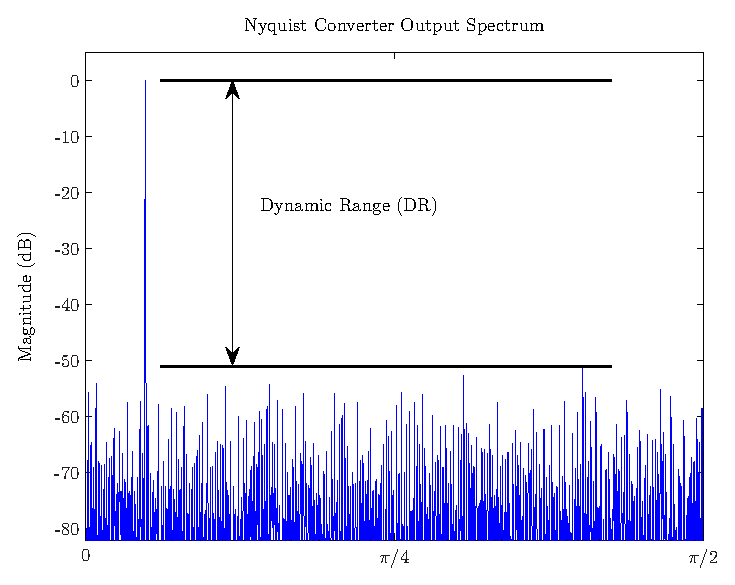
\includegraphics{./final_figures/nyquist_converter.eps}
 \caption{Nyquist Rate Output Spectrum (Dynamic Range)}
 \label{fig:nyquist_converter}
\end{figure}
%-------------------
The output spectrum clearly illustrates the superposited fundamental signal over the
quantization noise floor. Note that dynamic range is defined as the difference between the
largest component in the output spectrum, the fundamental signal, and the largest noise
element. If the noise floor were perfectly flat (i.e. no spurs or variation), the dynamic
range would be the difference between the power of the signal (typically normalized to
0 dB) and the average power of the noise. Alternatively, the SNR is equivalent to the DR
for a noise spectrum of perfectly equal magnitude over all frequency.

The noise shaping process introduces dips and rises in the noise floor of the operation
region of the \DSm due to the introduction of zeros and poles in the complex transfer
function which controls the NTF and STF. Thus, the DR will always be slightly less than
the SNR. This will be further illustrated in the following sections.